\section{Al jard'in de la Rep'ublica}

\subsection*{12 de Enero -- El Mollar}

Empezamos el viaje una ma\~nana temprano en Pergamino, mi viejo nos llevar'ia en
auto hasta Tucum'an Capital. 'El iba por trabajo, nosotros por decidido ocio.
Los 850~km se hicieron cortos, entre charlas y cambios de volante. Y, llegados a
la ciudad, el viejo no perd'ia oportunidad de invitarnos con comidas y
comodidades. El temporal que hubo nos sorprendi'o, a Dios gracias, bajo techo
con pap'a, as'i que no la pasamos muy mal. De hecho la pasamos bien, sin saber
que era tan grave. \textexclamdown Pensar que plane'abamos acampar!

Llegamos al siguiente mediod'ia a Acheral, en el sur de Tucum'an, donde
comenzar'ia el bicicleteo. La ruta recorrer'ia las selvas de Tucum'an,
atravesar'ia Salta por la Ruta Nacional 40, para finalizar --recorriendo la
Quebrada de Humahuaca-- en Iruya, destino final del viaje.

Mi viejo no quer'ia dejarnos, \textexclamdown segu'ia viaje con el auto a pesar
de que est'abamos pasando Acheral! Hasta se tom'o la precauci'on de comprar
chocolates de m'as en el almuerzo, para dejarnos lo que sobrara. \textexclamdown
Siempre bienvenidos!

Frenamos en la banquina y esparcimos todos los bolsos para empezar a acomodar.
Desde ah'i se ve'ia una larga recta en subida. El viejo observaba, y nos dec'ia:

\subparagraph{}\label{ssub:papa} --- \textquestiondown Saben lo que siento?\\
--- \textquestiondown Qu'e?\\ --- \textexclamdown L'astima!\\ \hangindent=1cm

Nosotros nos mor'iamos de risa mientras rearm'abamos las bicis y alforjas. Es mi
quinto viaje, pap'a conoce las fotos, pero nunca me vio alej'andome a pedal,
supongo nunca habr'a sentido c'omo se lo vive. Con Eze, a la inversa, nos
sorprendemos de que no todos sientan que viajar en bici es de pel'icula.
Guardamos los chocolates a mano, y subimos a las bicis. Recorridos nuestros
primeros metros pap'a dio la vuelta a Pergamino.

Este primer recorrido siempre es euf'orico, empezamos andando r'apido y
emocionados. Paramos a pedir agua en un rancho, ya que la indundaci'on la
hab'ia cortado en Acheral. Esta noche dormir'iamos en el monumento al Indio, una
estatua 40~km m'as arriba por esta ruta. Hicimos la larga subida acompa\~nados
por unos amigables chicos que nos vieron pasar por la entrada de su pueblo
(Santa Luc'ia), y pedaleaban a nuestro lado haciendo preguntas, a modo de apoyo
y compa\~n'ia. Les hab'ia llamado la atenci'on las grandes alforjas, y pensaban
que ven'iamos de muy lejos, \textexclamdown pero ah'i mismo empez'abamos el
viaje a la Quebrada! Uno se cay'o violentamente al cort'arsele la cadena
mientras hac'ia fuerza, tuvo que volver justo antes del Indio.

A pesar de nuestro cansancio --luego de un sedentario a\~no universitario--
pasamos el Indio, no parec'ia un lugar interesante donde acampar. Dos viajeros
en moto nos suger'ian llegar a El Mollar: aseguraban que el camino era
imperdible, de no muchos kil'ometros, y que el pueblo estaba bueno para salir a
tomar algo. \textexclamdown Se olvidaron que las subidas son obst'aculos para la
bici!

Cubrimos 53~km de subidas en curvas y selvas este d'ia, no tuvimos respiro.
Llegamos tan tarde y cansados a este pueblo (``Tafiloche'' le dicen,
tiene mucha joda) que nos quedamos dos noches. \textexclamdown Ni pudimos dormir
bien con la cantidad de cumbias distintas que se escuchan en el mismo
campamento! Ponen a fondo, saturando aunque est'en sentados charlando.
Content'isimos, una meta hermosa completar toda esa subida en un 'unico d'ia.
Tomamos unos fernet, y a la carpa.

El siguiente d'ia lo pasamos entre lluvias --menos mal que lo tomar'iamos de
descanso-- y lecturas. Ya termin'e un libro, y empec'e uno de Historia que est'a
muy bueno. Estamos comiendo como garzas, tan rico y barato. Las bicis llaman un
poco la atenci'on, hay muchos mochileros en colectivo por ac'a. Ni siquiera
viajan a dedo: \textexclamdown por esta ruta no hay lugar en las banquinas para
hacerlo!

Como no pod'ia ser de otro modo para un viaje nuestro: 'epoca de lluvias. Est'a
lloviendo hasta en Cafayate, t'ipicamente seco. Vamos a terminar viendo la
Quebrada con paisaje selv'atico entre tanto cambio clim'atico.

Caminos y lugares divinos hasta ahora, seguro despu'es tambi'en. Ma\~nana, a
Taf'i del Valle, unos 13 relajados kil'ometros. \textexclamdown Y luego, a
seguir subiendo!

\section{Paisajes y personas norte\~nas}

\subsection*{14 de Enero -- Taf'i del Valle}

Salimos para Taf'i cruzando un hermoso valle, unos 13~km de bajada. Una ciudad
de mucha belleza, a diferencia de El Mollar, donde lo interesante es s'olo la
gran joda que tienen. Comimos una sand'ia en una plaza (\textexclamdown
riqu'isima! La bautizamos ``porota''), recorrimos, llovi'o, nos instalamos en un
buen camping\ldots\ Un buen d'ia.

Conocimos a dos viejas de aqu'i que trabajaron con {\small PROSAP}, que
es un programa de desarrollo regional. Gracias a eso se capacitaron y
aprendieron a vender productos que antes s'olo hac'ian para ellos. La mujer
estaba muy contenta y orgullosa de los logros. Ofrec'ian en esa noche cazuela de
pollo a \$2,50; un estadounidense no podr'ia creer el estar comiendo un plato
rico (en plato de vidrio, de los cotidianos de una casa) a menos de un d'olar.

\subsection*{15 de Enero -- Amaich'a del Valle}

Salimos para Amaich'a del Valle, cruzando el muy famoso por ac'a ``Infiernillo",
el punto m'as alto de la provincia de Tucum'an. Pasamos de los 2000 a los 3000
msnm. Nos advert'ian que ah'i
nos morir'iamos de fr'io, pero subiendo transpiramos como en el Caribe. Las
fotos y camino son espectaculares: una subida zigzageante en la que nos
despeg'abamos del valle, para verlo desde puntos cada vez m'as altos. Cuando
llegamos a esa suerte de altiplano nos cubri'o una niebla que no permit'ia ver a
diez metros de distancia, y un fr'io intenso que nos hizo abrigar como en
Invierno. Metros despu'es llegamos al mirador ``Infiernillo'', no se ve'ia el
pretendido valle pero s'i las nubes --que ya hab'iamos pasado-- desde arriba,
iluminadas por el sol, como si las estuvi'eramos sobrevolando. Y luego, ya
cansad'isimos, La Bajada (la Cuesta de los Cardones), que nos transport'o
de nuevo hasta los 2000 msnm sobre los que se asienta Amaich'a. Es decir que
recorrimos 50~km para avanzar, y otros 2~km de desnivel.

El camino hasta ese punto era con vegetaci'on, pero desde El Infiernillo se
torn'o instant'aneamente 'arido, mostrando ahora cardos, piedras y burros que
corr'ian asustados a nuestro paso. Las casas son ahora de piedra y paja,
impresiona el abrupto cambio de climas y paisajes. Desde ahora podremos
olvidarnos --hasta la vuelta a las Pampas-- de las lluvias y humedad. Bajamos
esa Cuesta de los Cardones al atardecer, y fue uno de los momentos m'as
divertidos que viv'i sobre la bici. Tomados fuerte del manubrio avanz'abamos
sobre el viejo y roto pavimento entre empinadas curvas; y a nuestra derecha
pasaban las cercanas paredes monta\~nosas a gran velocidad; a la izquierda, los
postes que separan la ruta del precipicio, m'as suavemente; y, casi lentamente,
se alejaban las monta\~nas del otro lado del r'io que borde'abamos. Inolvidable.

Cuando sub'iamos nos adelantaron dos chicos en moto, no nos dejaron de
alentar, hasta que desaparecieron. Seguimos pedaleando, agradecidos por el
enchufe. Luego de nuestra bajada paramos a tomar agua en un descanso, y nos
volvi'o a cruzar la moto, que volv'ia ahora para Taf'i y le tocaba subir. Nos
saludamos, y cuando llegaron a la parte empinada\ldots\ \textexclamdown no
pod'ian avanzar! La pobre moto iba a toda m'aquina a 5~km/h, \textexclamdown los
chicos ten'ian que bajar los pies para empujar y no caerse, como los picapiedra!
Les empezamos a gritar:

\subparagraph{}\label{ssub:alentando} --- \textexclamdown Vaamos chicos, vamos
que pueden! \textexclamdown \textexclamdown Fuerza, fuerza muchachos que van a
poder!!\\ \hangindent=1cm

Nuestras voces hac'ian eco, nos mor'iamos de risa y los muchachos tambi'en.

La noche nos sorprendi'o en esta bajada, instalamos las luces 10~km antes de
la llegada: yo la roja atr'as, Eze la azulada (potente) adelante. Baj'abamos al
Valle acerc'andonos a la iluminada Amaich'a a 50~km/h, ahora casi en recta y con
menos curvas, separados por cent'imetros uno del otro para protegernos del
viento y por las luces complementarias. Cielo estrellado. Fue m'agico, es
indescriptible. El ruido de las cubiertas, el juego de zigzags para no chocarnos
y el sonido del viento en la oscuridad infunden una divertida emoci'on.

Llegamos en estado de euforia a la plaza central, dejando las bicis al lado de
una parrillita callejera que ofrec'ia excelentes choripanes. En la esquina donde
los engullimos con marcado placer hab'ia j'ovenes sentados en el bar, por sus
miradas a nosotros y a los bolsos sobre las bicis lograron hacerme sentir como
forastero, por primera vez en Argentina. Empec'e a notar lo diferente que es el
Noroeste de toda la Argentina que entonces conoc'ia.

Bien dormidos, al otro d'ia quisimos conocer El Remate --efusivamente
recomendado por un tucumano-- subiendo 8~km desde la Plaza central. Casi
lleg'abamos, cuando otros mochileros nos dijeron que la inminente lluvia lo
tornar'ia peligroso por la crecida del r'io; tuvimos que volver. Para colmo
hicimos la bajada en colectivo, porque pinch'e la primer rueda del viaje y no
llev'e herramientas. \textexclamdown Qu'e embole perder la bajada despu'es de
pedalear la subida! Subiendo tomamos lindas fotos con ni\~nos del lugar, nos
miraban extasiados, y a la c'amara como a algo de otro mundo. \textexclamdown Se
ve'ian y se re'ian! Divinos. Lo extra\~no es que a juzgar por la dentadura ya
ten'ian 60 a\~nos, \textquestiondown c'omo se da\~nar'a tan pronto?

De vuelta en el campamento, comimos sandwichs de milanesa a \$ 3 (con la excusa
de que es barato no cocinamos nunca). Fue un d'ia de lecturas, descansando
porque ma\~nana viajamos a las Ruinas de Quilmes, camino a Cafayate.

\subsection*{17 de Enero -- Ruinas de Quilmes}

Las Ruinas son conmovedoras. \emph{Toda} esa historia cruda y rica de los indios
Quilmes, los paisajes, el valle, la subida a la monta\~na y su fortificaci'on,
la vista a casi 360$^\circ$\ldots\ intentar'e describirlos en orden.

Se llega a la base de la monta\~na desvi'andose unos 4~km de la Ruta 40. La
monta\~na se levanta sobre la planicie como un sorpresivo muro: aqu'i sub'ian
para defenderse de los espa\~noles, que llegaban a caballo para someterlos.
Viv'ian la vida de paz alrededor, en sus casas de la planicie. La zona de la
monta\~na es lo 'unico reconstruido: la Universidad de La Plata arm'o paredes de
piedras perfectamente encajadas como anta\~no; lo dem'as son s'olo cimientos,
tapados por la escasa vegetaci'on.

Comenzamos a subir a pie, era como una escalera interminable. Cuando nos dimos
vuelta para ver d'onde est'abamos, vimos lejanas a la ruta y la planicie all'a
abajo, como si hubi'eramos ascendido en avioneta. Cansados, nos sentamos sobre
una pared de las ruinas a comer y tomar agua, pensando en toda esta historia.
Los indios Quilmes resistieron 130 a\~nos las embestidas colonizadoras: arriba
en la monta\~na hay una excelente visibilidad a lo lejos, parece facilitar la
defensa y el ataque, mucho mejor que a caballo desde abajo y sin
fortificaciones. La historia estremece: durante las batallas las madres se
tiraban al precipicio del otro lado con sus beb'es; luego de esclavizados
emprendieron una marcha hacia Buenos Aires, los pocos que llegaron a la actual
Quilmes (a unos 1500~km de aqu'i), evitaron la reproducci'on, y as'i se
extinguieron.

Recorrimos todas las ruinas, y bajamos al atardecer, hora de armar campamento.
Al volver por el desv'io hacia la {\small RN}40, tomamos otro camino
paralelo a la ruta pero de piedras y arena, dif'icil de transitar sobre las
bicis, que nos adentraba en un desolado monte, ocupado por pocos burros y por
arbustos bajos. Armamos campamento en un llano, entre la cadena monta\~nosa de
las ruinas y un peque\~no morro que nos separa de la ruta. Fue una noche
simplemente emocionante. \textexclamdown En ese mismo suelo hab'ian estado los
caballos y ej'ercito colonizador, intentando vencer a estos nativos!
\textexclamdown Ese mismo suelo, donde ahora cen'abamos una buena picada, antes
de pasar una tranquila noche!

\begin{center}
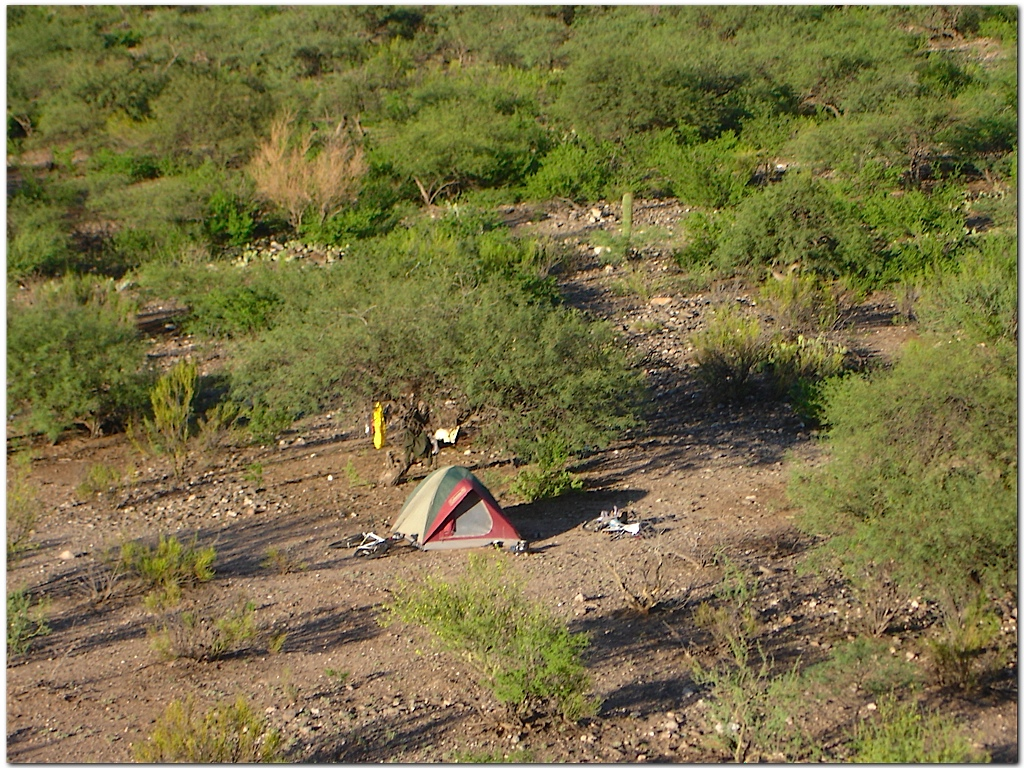
\includegraphics[width=300px]{images/DSC0123.JPG}
\textsc{\\``Camping libre.''}
\end{center}

\subsection*{18 de Enero -- Cafayate}

Desayunamos sobre el morro, observando tanto a las ruinas como a la ruta
mientras sub'ia el sol. Preparamos las alforjas para seguir a Cafayate. Ya en
camino, pasamos varios r'ios que atraviesan la ruta. Cruz'abamos Colalao del
Valle cuando decidimos parar a almorzar en su hermosa plaza central. Compramos
mont'on de verduras para armar una suculenta ensalada de todo, con condimentos
prestados por un due\~no de casa.

Pretend'iamos pasar la siesta para evitar al gran sol, pero, inquietos como
siempre, decidimos seguir pasado un ratito. A las pocas cuadras encontramos a
dos grandes viajeros en bici, bajo la sombra de los 'arboles. El calificativo de
``grandes'' se lo dan la apariencia de extranjeros lejanos, las banderas sobre
las bicis, las alforjas atr'as y adelante y el bob (carrito con bolsos tirado
por la bici). Se trataba de norteamericanos que hablaban buen espa\~nol. Greg
viaja desde Alaska a Ushuaia en beneficio de una fundaci'on
(\texttt{http://www.ribbonofroad.com/}), y Tom, estudiante de Geograf'ia, se
prendi'o en Quito, Ecuador, al pedaleo. Charlando nos morimos de risa por dos
horas, hasta que dieron las 4pm y siguieron viaje. Contaban unos relatos
impresionantes, dif'icil de seleccionar, pero me interesa por ejemplo que en el
desierto boliviano tenian que mandar comida en jeeps a los paradores, porque en
ese momento eran 5 viajeros y las proveedur'ias, casi fantasmas asentadas sobre
un camino tur'istico abandonado, no ten'ian provisiones para todos. En una, el
due\~no, al ver que le compraban literalmente todo por 100 o 200 soles, les dijo
que con 200 m'as les dejaba el negocio. \textexclamdown Embolado de vivir ah'i,
solo, cruzando a algun que otro loco dolarizado! Les vend'ia su lugar por poco
m'as que su mercader'ia. Muchas otras historias, como se imaginar'an; por la
onda le sugerimos al compa\~nero de Greg que conozca El Mollar.
``\textexclamdown Buen viaje!", y a la ruta en sentidos opuestos.

Bajadas y subidas de por medio, llegamos a Cafayate, muy pintoresca ciudad,
donde paramos en un camping medio caro en busca de buenos ba\~nos y duchas. Y
hoy, descanso y a pasar el d'ia en la pileta, esperando a nuestro amigo y
compa\~nero Sergio, profesor de Educaci'on F'isica de la Universidad de La Plata
de unos 50 a\~nos, que viene un d'ia desfasado. Ma\~nana empezamos juntos la
ruta a Cachi, me cago todo porque hasta estos grandes viajeros en bici me dicen
que ``la 40'' no es cosa f'acil.

\subsection*{19 de Enero}

Hoy seguir'iamos hacia Cachi, pero Sergio, llegado ayer, nos tent'o de
quedarnos. \textexclamdown El loco viene muerto porque le exigimos que se apure!
Dice que le ment'i, que no es dif'icil la subida de Tucum'an, \textexclamdown
sino que es ``dificil'icima''! Salimos a cenar, y luego de esperar una hora una
pizza\ldots\ \textexclamdown terminamos comiendo dos lomos completos cada uno en
un kiosquito cercano! \textexclamdown Y no nos movemos! Como lo invitamos, ahora
nos quiere invitar al almuerzo, venimos aliment'andonos como pavo antes del d'ia
de acci'on de gracias.

No quiere tocar la bici, as'i que paseamos a pie por la ciudad. Hoy vamos en
auto a la Quebrada de las Conchas, veremos de qu'e se trata, para ma\~nana s'i
continuar por la serruchada y enripiada {\small RN}40; no hay quien nos
tire buena onda pero ya veremos qu'e nos depara. Estamos expectantes,
\textexclamdown creo que nos va a cansar y a gustar mucho!

Yo ven'ia con miedo porque mi bici no anda muy bien: la cadena giraba en falso.
Luego de visitar dos o tres bicicleter'ias que me mandaban a Salta Capital
(imposible), porque ac'a hay viejos pi\~nones a rosca y no a cassette, termin'e
en la casa de un corredor de bicis, que se di'o ma\~na y con un buen trabajo de
limpieza la dej'o nueva. Cobr'o una m'odica mano de obra, y me salv'o buena
parte del viaje. Profundamente agradecido.

\subsection*{24 de Enero -- Cachi}

En estos d'ias completamos el viaje desde Cafayate a Cachi, no por Salta Capital
sino por la m'itica para nosotros ``cuarenta'', algo completamente inolvidable.
Pasamos por cuatro pueblitos perdidos (San Carlos, Angastaco, Molinos y
Seclant'as) que, me animo a decir, son los lugares que con m'as exactitud y
cari\~no recuerdo. Si se viaja con 'animos de conocer cultura, estos puntos
perdidos y sin inter'es tur'istico son el centro y nudo del viaje.

La Ruta impacta, no pasaba un alma. Desde San Carlos casi comienza el ripio,
'este es un pueblo que recuerda (por pel'iculas, pues no conozco) a M'exico,
antiguo y hermoso. Almorzamos aqu'i media docena de riqu'isimas y pesadas
empanadas salte\~nas (salte\~nas porque tienen papa hervida). No s'e como mi
boca sobrevive sin quemarse. Pedimos por el ba\~no y, muy amablemente, nos
condujeron por un largo corredor al patio central y privado, donde estaba el
precario ba\~no de los cocineros, los due\~nos de casa. Qu'e simple y gran
atenci'on a las personas (aunque en este caso fu'eramos clientes).

Hasta Cachi el ripio continu'o como empez'o: serruchos, suelo un tanto arenoso,
y muchas curvas y desniveles. \textexclamdown Un camino para no aburrirse! Se
cansan las piernas, pero no mucho m'as que la espalda, los brazos y el cuello.
Cruzamos algunos vados embarrados, 'este es en verdad un viaje para la bici. Los
paisajes cambian cada 5~km, uno no puede cansarse de mirar, en toda direcci'on y
momento.

Sergio casi muere, lleg'o descompensado. Es que fue un d'ia muy duro entre el
viento en contra y la dif'icil ruta, pero la emoci'on de estar haciendo
exactamente lo que quer'iamos no nos permiti'o decaer. La noche nos sorprendi'o
en camino, luego de dos pinchazos (durante el viaje pinchamos incontables
c'amaras, debido al peso, estado del camino, y baja presi'on con que
err'oneamente las infl'abamos), y sin embargo con Eze no sent'iamos buen humor,
sino una muy concreta euforia: salimos de Pergamino buscando \emph{esto}. Un
cielo netamente estrellado, y la luna est'a creciendo aunque casi no existe.
Bajamos la Quebrada de las Flechas --zona del camino donde se aprecian
indescriptibles formas que la erosi'on le imprimi'o a las monta\~nas-- a tal
velocidad que no nos permitimos detenernos para tomar fotos. Son los caminos que
esper'abamos.

Cuando vimos el cartel del desv'io a Angastaco s'i que nos detuvimos y, mientras
el extenuado Sergio enfocaba en la plena oscuridad, con Ezequiel nos
acomod'abamos detr'as del cartel planeando hacerle alg'un otro chiste. Nuestras
risas no le provocaron sospechas, y cuando dispar'o el flash retrat'o grandes y
blancos no nuestros dientes, \textexclamdown sino nuestros respectivos traseros!
Le preguntamos si salimos con mala cara, y entre carcajadas volvimos a subir a
las bicis para completar el desv'io al pueblo.

Llegamos a Angastaco de noche cerrada, con mucho cansancio y altos 'animos. Es
un pueblo m'inimo, con un campamento, su plaza e iglesia, una lujosa hoster'ia,
y muy poco turismo. Aqu'i por segunda vez me sent'i forastero dentro de ``mi''
propio pa'is. Llegamos a las 22:30, y lo que nos un'ia a los lugare\~nos
(reunidos en esta noche de s'abado alrededor de la plaza principal) era
'unicamente el partido River-Boca, que se proyectaba en el barcito dos cuadras
m'as arriba. Y tambi'en, claro, sus atentas miradas hacia estos ruidosos
viajeros.

Comimos en el barcito un delicioso matambre tiernizado, y tomamos una buena
cerveza. Divertida charla, y a medianoche salimos a buscar campamento. Pedimos
ayuda a unos j'ovenes que tomaban cervezas en una puerta de casa, y nos
acompa\~naron caminando hasta donde viv'ia el cuidador del campamento, quien
descansaba apaciblemente pero le interrumpimos, pidiendo que nos acompa\~ne a
nuestros aposentos. Agradecimos mucho a los j'ovenes, quienes, con la misma
simpleza con que nos ayudaron, se despidieron y volvieron a su vereda. El
hombre nos abri'o unos particulares bungalows, donde descansamos luego de darnos
un potente ba\~no. Desde una ducha Sergio suspiraba en su cansancio como si
estuviera d'andose un ba\~no de inmersi'on, \textexclamdown lo imit'abamos
exagerando y las risas se escuchaban en todo el camping!

Dormimos muy bien, y al levantarnos jugamos un picadito con ni\~nos del lugar,
nos miran como si vini'eramos del planeta Saturno. Luego Ezequiel y yo seguimos
hacia Molinos, y Sergio se qued'o a hacer vida de paz en Angastaco, lavando ropa
y acomodando la bici, que se le rompe m'as que la m'ia.

\begin{center} 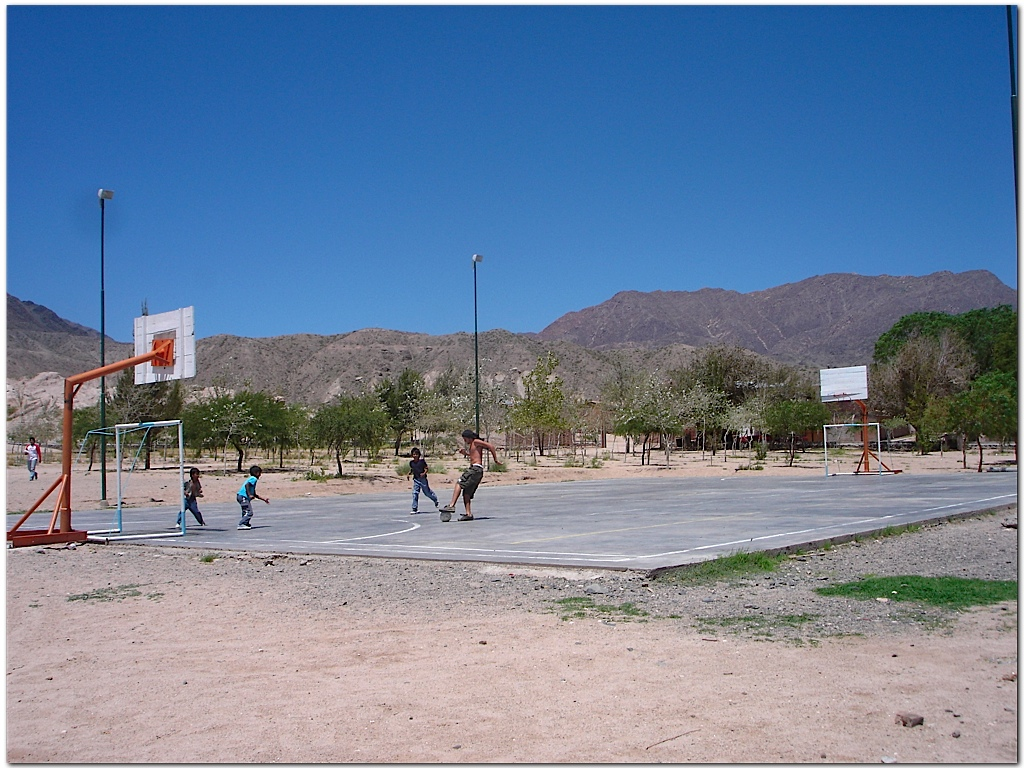
\includegraphics[width=300px]{images/DSC0194.jpg}
\textsc{\\F'utbol en Angastaco.} \end{center}

Camino a Molinos cruzamos tres turistas: uno era alem'an, de unos 27 a\~nos. Le
pregunt'e de d'onde es y me contest'o muy sonriente que viene de un pueblo
cercano a \emph{Hannover}.

\subparagraph{}\label{ssub:gottingen} --- \textexclamdown Mir'a vos! Yo viv'i
dos meses en G\"ottingen.\\ --- Bueno, \textexclamdown de ah'i soy!\\
\hangindent=1cm

Le pregunt'e por Gustav y por Axel, nombrando calles, y con cara de incr'edulo
me contestaba que no los conoc'ia. No dejaba de repetir ``\emph{it's
incredible}'', y la verdad que lo era.

El viaje fue muy sabroso, recorriendo una angosta ruta serpenteante, con tantas
cortas subidas como bajadas, precipicios a veces sin guardariel, entre aridez,
arboledas, cultivos regados por acequias, y monta\~nas. Pocos veh'iculos.
Encontramos a un lugare\~no sentado a la vera de la ruta, solo, vestido de
pantalones largos y camisa; y le ofrecimos agua seguros de su soledad, pero nos
indic'o su casa bajo la ruta. Esa familia viv'ia ah'i, incomprensible para
estos viajeros citadinos. Agradecido, nos dese'o un buen viaje. Yo no me detuve
hasta pocos kil'ometros antes de Molinos, donde par'e a esperar a mi
compa\~nero, sentado en un tronco frente a una casa de barro y paja.

Apoy'e la bici sobre la banquina y mir'e al camino, descansando. Se acercaron
dos ni\~nos de la casa interesados por mi viaje, y les empec'e a contar todo,
miraban con ojos grandes. Parece que esperaban con tanta ansiedad a Ezequiel
como yo, porque cuando lleg'o le demostraron m'as alegr'ia que yo mismo,
\textexclamdown se compenetraron con la historia!

Nos pasamos todo el atardecer jugando con otros hermanos y primos suyos, nos
contaron que ven'ian a esta casa a hornear el pan, nos ense\~naron la vista que
tienen desde arriba del cerro, y tomamos mont'on de fotos que nos hac'ian reir a
todos. Lo gracioso es que se sorprend'ian ante el paso de cada avi'on, y nos
escuchaban y miraban interesados, pero no les sorprend'ia la bicicleta m'as que
cualquier auto porque por esta ruta pasan, justamente, muchos viajeros de todo
tipo. Y como todos los ni\~nos de estas zonas, se alegraban tant'isimo de que
tuvi'eramos caramelos o galletitas dulces para compartir. Al bajar del cerro a
buscar pilas para la c'amara la madre sali'o t'imida de la casa, y nos regal'o
un pan reci'en sacado del horno, menos mal porque le com'ia un chico sino. Fue
hermoso. Despedirnos no fue tarea f'acil: cuando logr'abamos bajar a las
ni\~nitas --que apenas pod'ian caminar-- de las bicis e intent'abamos subir,
\textexclamdown se volv'ian a trepar! Agradecimientos, y a Molinos.

Molinos es un pueblo hermoso. Dej'e todos los bolsos en el camping y salimos a
comprar provisiones. \textexclamdown Era una moto! \emph{A fondo} por todo el
pueblo, me di cuenta de que tengo que limpiar los pobres frenos porque no
frenaba tanto como aceleraba. Me acostumbr'e al equipaje, y me vuelvo a sentir
como andaba en la secundaria: completamente liviano.

Al llegar al camping con las provisiones encontramos a los mismos chicos del
atardecer, viven por ah'i. Un poco vergonzosos, nos pidieron las bicis, y en
cuanto escucharon la primer letra del ``s'i'', se subieron y empezaron a hacer
carreritas en la calle de entrada del camping, se mor'ian de risa y no lo
pod'ian creer. Comieron de nuestra polenta, y se fueron a dormir cuando los
echamos; tambi'en nos 'ibamos a dormir.

A la ma\~nana hicimos una caminata larga por todo Molinos con un gu'ia del
lugar, muy buena. Conoc'i la tumba de quien descuartiz'o a Tupac Amar'u; el
antiguo hostal es de un descendiente directo de este espa\~nol de apellido
Isasmendi, quien vive ahora en Salta.

Ten'iamos dos caminos a Seclant'as, el 'ultimo de esta seguidilla de
tradicionales pueblos: el largo y el corto, el ``f'acil'' y el ``duro". Elegimos
el corto y dif'icil por la emoci'on de la bajada, y la disfrutamos; pero los
10~km de constante subida se hicieron largos, as'i que preferimos el otro, con
curvas y desniveles m'as constantes.

Telares y tapices por doquier, paramos en la casa del primer telar que vimos y
quer'iamos charlar con una vieja, pero no nos daba bolilla. Nos empezamos a
asustar: se acercaba sin emitir un sonido, y casi ni nos miraba\ldots\
\textexclamdown y es que era ciega y sorda! Nos escuch'o el hijo y nos explic'o,
casi morimos de un espasmo hasta ese momento.

Llegamos al camping, su due\~na y los dem'as acampantes nos trataron tan
amigablemente como cualquier viejo amigo. Aqu'i vimos por primera vez a una
norte\~na vestida t'ipicamente, y ella se sorprendi'o tanto de nuestra actitud
de pretender tomarle una foto, como nosotros de su vestimenta y de su caminata
con pesadas bolsas, a pesar de la avanzada edad.

Conocimos el cementerio, es t'etrico. El peor cementerio que conoc'i es el de
Seclant'as, peor a'un que el abandonado de Manuel Ocampo, cercano a Pergamino.
Sin planificaciones, atestado; uno entra y se choca dos tumbas, no hay caminos,
se anda por encima de ellas, los nichos son una desprolijidad\ldots\ desolador.
Se puede entrar a dos mausoleos de poderosas familias sin necesidad de entrar al
cementerio: est'an al costado y separados, y se ven a'un m'as que la propia
iglesia. Muy raro.\\

La distancia corta que recorrimos este d'ia permiti'o que Sergio nos alcance al
otro d'ia, as'i que, luego de nuestra noche en Seclant'as, salimos juntos hacia
Cachi. Recorrimos la ruta de los Artesanos, donde conocimos --entre otros tantos
(inhibidos como muy abiertos)-- al Tero Guzm'an justo en el d'ia de su
cumplea\~nos n'umero 77, el 23 de Enero. Le hizo ponchos a Juan Pablo II, Lula
da Silva, los Chalchaleros, y contando. Ya est'a un poco viejo para el trabajo
as'i que tiene a los nietos de ac'a para all'a. Le compr'e un cinto para mis
bermudas que queda de diez. Paramos en otros tres telares, y pinchamos otras dos
cubiertas adem'as de cambiar un cable cortado, por lo que la noche nos volvi'o a
sorprender.

Al atardecer, unos lugare\~nos de San Jos'e hab'ian armado una canchita de
f'utbol a lo largo de la ruta con rocas, \textexclamdown qu'e bueno! Tuvimos que
interrumpir su picadito: ``\textexclamdown perd'on que nos metamos en el campo
de juego, muchachos!'', nos re'iamos todos.

Nos rodeaba una violenta tormenta el'ectrica que por suerte no se posaba arriba
nuestro. Pedalear esos serruchos de la ruta, en medio de aquellas constantemente
iluminadas nubes de la noche, fue emocionante, aunque yo estaba asustado entre
la inminente tormenta, la oscuridad y los perros que a veces nos persegu'ian
ladrando.

\begin{center} 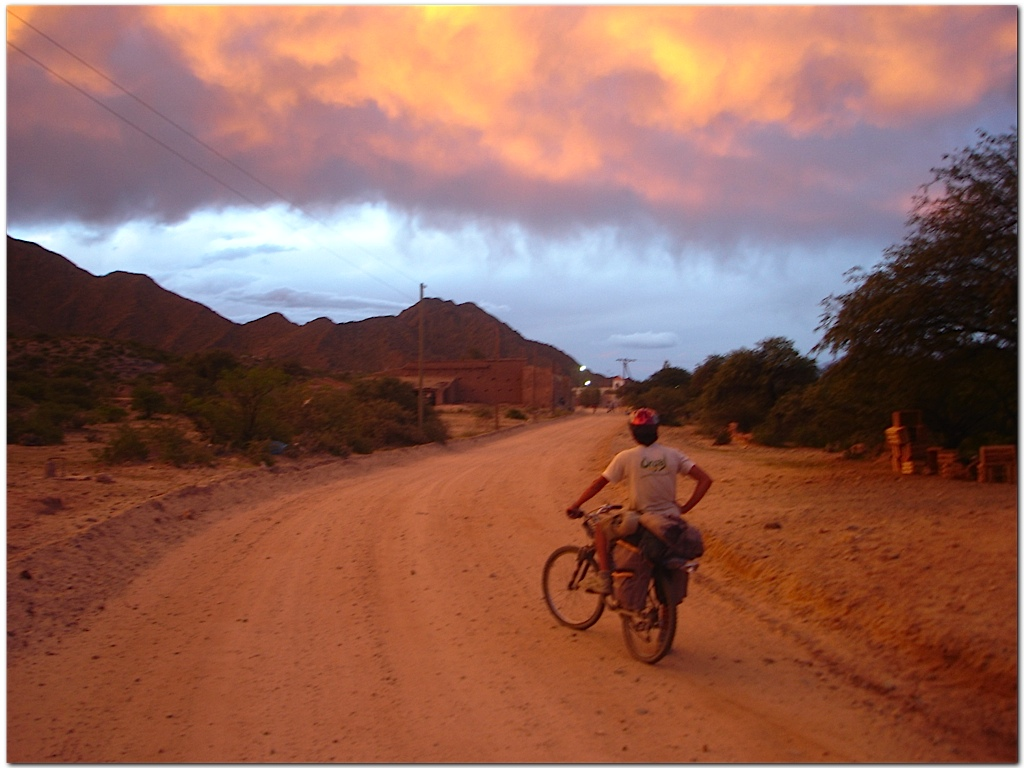
\includegraphics[width=300px]{images/DSC0296.jpg}
\textsc{\\Entrando a San Jos'e, bajo nubes po'eticas o infernales.}
\end{center}

La llegada a Cachi signific'o para mi un gran alivio. Bajamos por una de sus
calles hasta la plaza central, donde ahora nos esperaba Sergio, quien hab'ia
llegado directo por la 40 (sin artesanos: desviarse implicaba la noche en el
camino). Nos indicaron un hermoso comedor, donde ofrec'ian buenos y r'apidos
lomos, y mientras los disfrut'abamos se desat'o la instant'anea tormenta de
verano: lluvia a baldazos y unos rayos y truenos que hac'ian temblar la tierra;
nunca los escuch'e tan fuertes como en el Norte. Agradecidos de que no nos
sorprendiera en el medio de la ruta, terminamos el lomo y la tormenta de verano
pas'o, ahora se ve'ian las estrellas. Impredecible.

Bonito camping y buen descanso, nos tomamos un d'ia para recorrer esta
hermos'isima ciudad colonial, respirar, enviar noticias, tomar un aperitivo, y
las cosas que se hacen cuando uno se baja de la bicicleta. Toda la gente de lo
mejor, de diez. Los precios, norte\~nos, hasta llegar a Cachi que tiene ruta
pavimentada desde Salta.

\section{Pedaleando por las nubes, el Abra del Acay}

\subsection*{28 de Enero -- Al Abra del Acay}

Hoy nos separamos de Sergio en Payogasta, cerquita de Cachi: su viaje culminaba
en Salta bajando por la Cuesta del Obispo, pero el nuestro continuaba al Norte
por la 40. A la sombra de un gran 'arbol nos desped'iamos con una interminable
cola de chistes, hasta una vieja espectadora sonre'ia. Una canilla solitaria y
muy oportuna nos provey'o de agua. Lo vimos alejarse por el asfalto, y nosotros
continuamos en sentido contrario, luego de asegurar que se tratara de nuestra
ruta preguntando a la entretenida mujer.

Estamos expectantes porque nos acercamos al Abra del Acay, el punto m'as alto de
nuestras rutas Nacionales, que alcanza casi 5000 msnm. De lograr cruzarlo,
llegaremos bajando a San Antonio de los Cobres. Esper'abamos poco de esta ruta
desierta, sin embargo la altura, la inmensidad de las monta\~nas, y algunos
verdes valles se mostraron imponentes.

\begin{center} 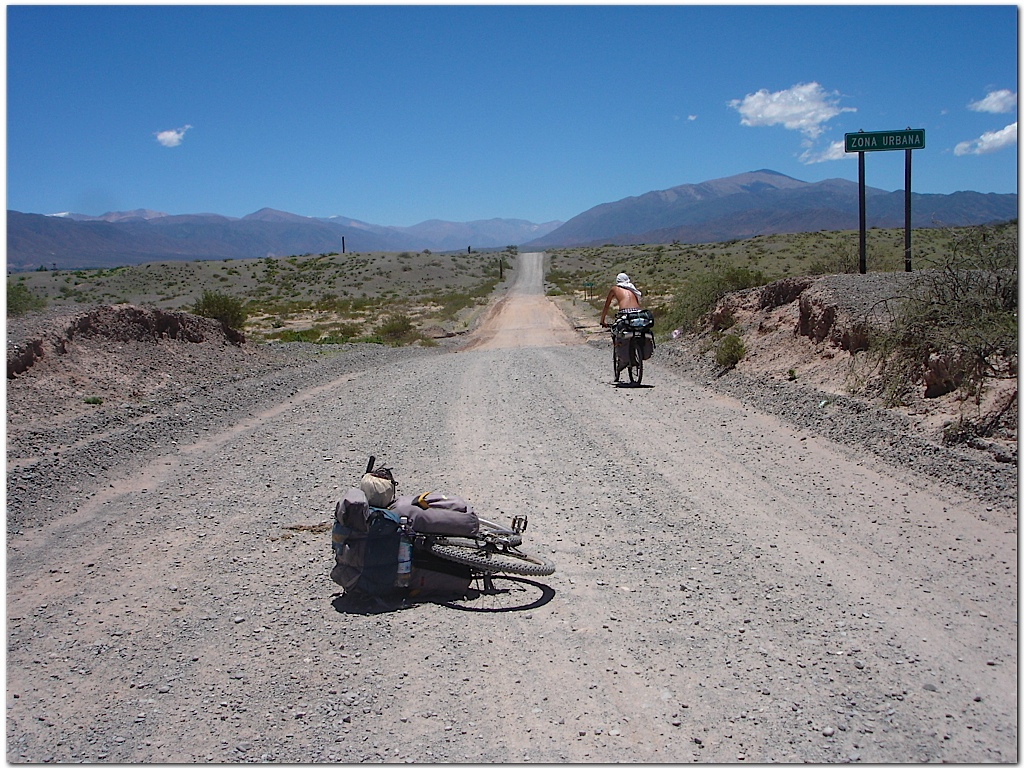
\includegraphics[width=300px]{images/DSC0311.jpg}
\textsc{\\``Zona urbana''. La bienvenida a la ruta desierta.} \end{center}

Pasamos el ``Pueblo Viejo'', y cruzamos por el camino a una muy avejentada mujer
que esperaba en la banquina. No pod'ia moverse ni hablar con facilidad, estaba
tan vestida que no entiendo c'omo no se deshidrataba del calor, y, sin embargo,
se mostraba muy interesada en charlar con nosotros, y no pod'ia borrar su
sonrisa. Ten'ia a su costado pesadas bolsas. Luego de una corta charla le
dejamos un paquete de galletitas dulces. Un encuentro irreal.

En todo el d'ia nos adelant'o un 'unico veh'iculo, y m'as tarde lo vimos volver
por donde ven'ia. Paramos a merendar sobre el camino, donde encontramos una
buena vista al r'io, dejando las bicicletas y bolsos desarmados sobre la
mism'isima Ruta 40. \textexclamdown Si pasaba alg'un veh'iculo, est'abamos
seguros, no tendr'ia m'as de dos ruedas!

Llegamos cansados y al atardecer al desv'io a La Poma, ciudad donde
dormir'iamos. \textexclamdown Esos 7~km (de desv'io) fueron los m'as largos de
todo el viaje! La Poma es un lindo y peque\~no poblado minero, asentado a los
pies de los volcanes extintos ``Gemelos", y habitado por pocos lugare\~nos y
otros tantos turistas (todos de aventura). Parece que aqu'i no se conoce turismo
``normal'', sino ciclistas, caminantes, y conductores de 4x4 ``extremos''; aqu'i
las alforjas no llaman la atenci'on.

Cenamos muy bien a las 8pm en un lugar que no ten'ia cartel, por esta zona
parece moneda corriente, este cyber tampoco tiene. Nos dimos un buen ba\~no
(que ansiaba desde hac'ia cuatro d'ias), y cenamos otra vez a medianoche, en la
posada, esta vez capeletinis.\\

Dormimos en camas con s'abanas, nos despertamos, y a desayunar y charlar con la
due\~na del lugar.

Nos cont'o sobre Damiana, una viejita que vive con su hija en ``La Negra
Muerta'', una casa construida 10~km antes del Abra. Nos aconsej'o firmemente que
paremos all'i y que no intentemos cruzar hoy, porque muy posiblemente nos
sorprenda la noche, y acampar en alturas parece tan peligroso como intentar
bajar a oscuras y debilitados; no hay chances. Nos dec'ia que Damiana estar'ia
encantada de recibir compa\~n'ia; y nosotros, encantados por conocerla,
aceptamos con ganas parar hoy all'i.

En La Poma hay gente un tanto reservada, \textexclamdown a algunos les costaba
responder a nuestras preguntas sobre el camino! Tambi'en los hay charletas, como
el due\~no de la proveedur'ia, al que no pod'iamos callar y nos retrasaba la
salida. \textexclamdown Miles de interesantes historias que contar sobre
viajeros y este particular cruce monta\~noso!

La ruta desde La Poma al Abra (y luego a San Antonio de los Cobres) es la que
imposibilita el tr'ansito de veh'iculos, con 4 cortes por r'ios y 2 por
derrumbes. Uno de los cortes por r'io ten'ia una ca'ida de 1 metro de alto.
\emph{Muy} divertido para atravesar con las bicis. A veces la ruta se pierde en
el lecho del r'io, y si uno lo sigue, unos cuantos metros m'as adelante vuelve a
encontrar la senda de ripio. La dificultad aqu'i era avanzar y no buscar el
camino, pues la ruta corre siempre por el valle exceptuando el Abra, donde se
unen las cadenas monta\~nosas y las atraviesa por arriba.

Los mojones, que deber'ian contar alrededor de 4600~km, presentaban inexplicable
y repentinamente ``escasos'' 1800~km, nos hac'ian sentir impotentemente perdidos
en medio de una lejana e inaccesible Cordillera. Soledad casi absoluta, excepto
por algunas cabras y su respectivo pastor.

No llegamos a lo de Damiana, armamos campamento al lado del r'io. Cenamos bien,
y dormimos ya sintiendo la falta de aire. Al levantarnos nos sorprendimos por la
escarcha que se form'o sobre la carpa. Dos locos estaban haciendo el camino a
pie, no se esperaban la ausencia de autos. Locos, \textexclamdown literalmente!
Nos encontraron esta ma\~nana, y desayunamos juntos. Les alivi'o nuestro t'e:
ven'ian muertos de fr'io y con los pies mojados (nosotros nos salvamos cruzando
los vados sobre las bicis).

Pretendimos conquistar el Abra esa siguiente jornada. Luego de mucho subir
encontramos una viejita muy parecida a una vela oscura derretida, bajaba
caminando y tejiendo de la monta\~na, rodeada de unos cuantos perritos. Le
pregunt'e si ella era Damiana (efectivamente ella era), y entonces pregunt'e si
est'abamos lejos de su casa, pero ``ahicito nom'as'', a la vuelta de la curva,
encontrar'iamos su casita. Irradiba una paz religiosa, mientras sus perritos no
nos dejaban de ladrar. Nos dec'ia sin dejar de tejer que est'abamos a tres horas
del Abra del Acay, y que lograr'iamos cruzar antes del atardecer, que
sigui'eramos. Pod'iamos parar en su casa, pero no encontrar'iamos a nadie.

\begin{center} 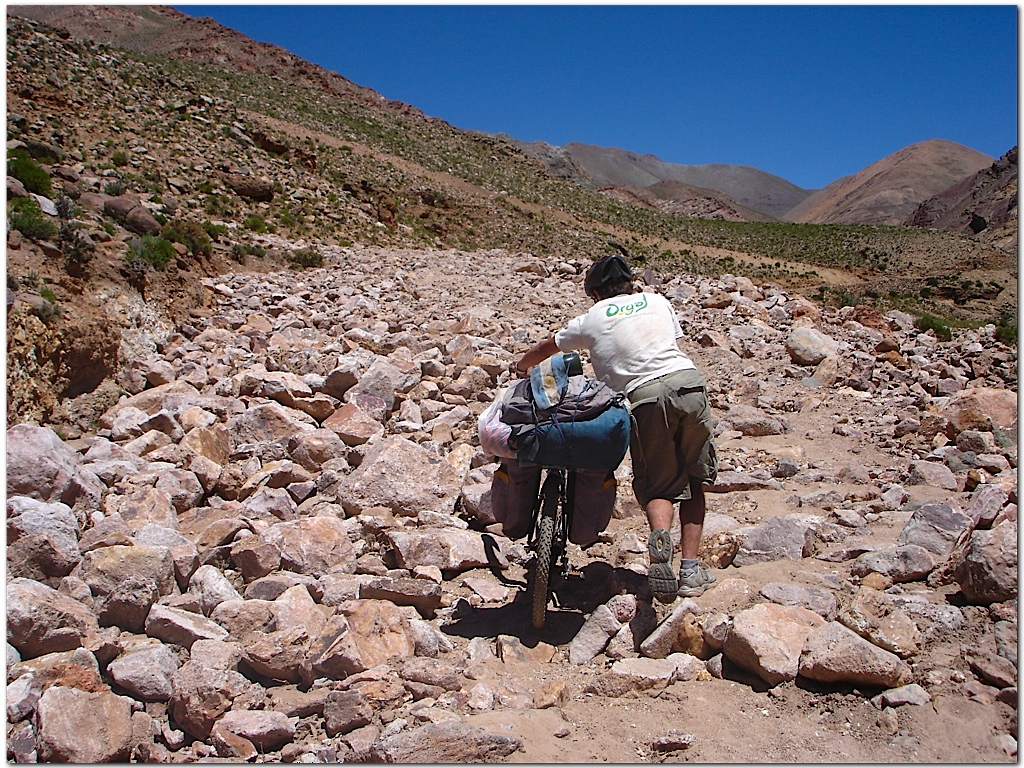
\includegraphics[width=300px]{images/DSC0369.jpg}
\textsc{\\Derrumbe sobre la Ruta 40.} \end{center}

Nos despedimos y continuamos el pedaleo. Pasamos por su casa, donde dejamos a la
vista nuestras galletitas para los dos caminantes, seguros de nuestro cruce.
Subimos mucho, nos cansamos moralmente: horas de subidas y curvas, paisajes
siempre iguales, cada vez m'as falta de aire, \textexclamdown el viento en
contra! Despu'es de cada curva esper'abamos ver la bajada, pero se demoraba
invariablemente. Continuamos sin que importe el paso de las horas: ten'iamos que
cruzar o volver para evitar el campamento en alturas.

Yo iba adelante, esperando poder anunciar la buena noticia a Ezequiel, y poder
levantar los 'animos. Y entonces, luego de una curva, lo vimos. Fue
desesperanzador. Estaba lejano, alt'isimo, subiendo una monta\~na por el camino
haciendo eses. Si cada veinte pasos --ni hablar de pedalear-- par'abamos a
tomar aire, probablemente llegar'iamos a medianoche, o ni lo lograr'iamos.
Desanimados, nos tiramos en la banquina. Abr'i una lata de carne y empec'e a
comer, no era agradable pero estaba hambriento. Ezequiel, asqueado, prefer'ia
evitarlo. Lo obligu'e a comer: ``Eze, uno de los s'intomas del apunamiento es
falta de hambre, justamente cuando m'as lo necesit'as. Comelo igual, dale''.
Pero lo vomit'o, sinti'endose cada vez peor. Me empec'e a desesperar:
\textquestiondown qu'e hacer? Somos inexpertos, \textquestiondown qu'e se hace
en estos casos? \textquestiondown Dormir en las alturas? \textquestiondown
Seguir, para poder luego bajar a San Antonio y comer a los m'as amigables
3700msnm? \textquestiondown Volver por donde vinimos, volver a La Poma? Ya no
quedaba suficiente agua y alimentos para alargar el viaje.

Durante esos pensamientos bajaban dos espa\~noles en bicicleta, reci'en hab'ian
cruzado en sentido inverso. Nos confirmaron que no llegar'iamos antes de la
fr'ia noche, restaban a'un 5~km. Aunque lleg'aramos, no ten'ia sentido describir
semejante bajada en las penumbras; deb'iamos hacerlo bajo el sol. Describimos el
camino de bajada que les esperaba, y nos dejaron un poco de agua, necesaria y
salvadora. Agradecimos, y siguieron bajando velozmente.

Intentaba preguntar a Ezequiel qu'e prefer'ia, pero le costaba pensar y
responder. Se sent'ia borracho, mareado al cerrar los ojos y con movimientos
poco exactos. Decid'i bajar un tramo, hasta alguna cueva formada por la
monta\~na donde armar la carpa y dormir. Si nos despert'abamos sinti'endonos
peor, volver'iamos sobre nuestra huella, y en caso contrario, la siguiente
ma\~nana seguir'iamos. Volvimos un par de kil'ometros, yo sent'ia miedo. En una
curva de 180$^\circ$ de unos caracoles que describ'ia el camino, contra la pared
de la monta\~na, armamos precariamente la carpa. Me acost'e en la bolsa de
dormir, vestido, pensando en que hab'iamos regalado provisiones seguros de
nuestra cena en San Antonio, pero nos tocaba este imprevisto cambio de planes. A
pesar de los minutos que transcurr'ian de descanso f'isico (pero no mental), mi
coraz'on no se calmaba, sent'ia taquicardia estando completamente quieto. Una
sensaci'on totalmente nueva e inquietante. Me asustaba el hambre y apunamiento,
lo que nos esperar'ia en el largo d'ia de ma\~nana, c'omo se sentir'ia Ezequiel
y yo, qu'e desayunar'iamos (sin hablar del est'omago vac'io de mi
compa\~nero).

Dormimos bien, a pesar del muy irregular y duro suelo rocoso. Nos despertamos a
las 8 de la ma\~nana al calor del sol. Abrimos la carpa y salimos, a'un
atontados por el profundo sue\~no. La sorpresa fue grande al vernos en medio
de ese imponente paisaje, peque\~nitos, luego de haber subido los caracoles que
se ve'ian hacia abajo, por subir los que nos esperaban adelante, y al costado
del profundo valle por donde bajaba un a'un peque\~no curso de agua, que
despu'es crec'ia. Levantarse as'i en el medio de la nada, pero de esos Paisajes,
es algo que no se puede describir. \textexclamdown Una sensaci'on moment'anea y
muy intensa!

Nos sent'iamos un tanto mejor f'isicamente, por buena suerte. Desayunamos leche
en polvo con la no mucha agua que quedaba. Mientras Eze terminaba con su
equipaje me recost'e sobre una roca, cerrar los ojos me acercaba casi
instant'aneamente al mundo de los sue\~nos. Y encaramos los 7~km que faltaban a
las 9:15 de la ma\~nana. Se sucedieron horas de profundo desgaste f'isico y
psicol'ogico, y sorpresa por nuestro ininterrumpidamente acelerado coraz'on. Sin
embargo, ahora pod'iamos ver desde arriba a las cadenas monta\~nosas que antes
rode'abamos subiendo impotentemente, y al pasarlas con la mirada pod'iamos ver
las distintas cadenas que se suced'ian. Luego de muchas horas de tener la vista
interrumpida por paredes, uno puede observar desde arriba a esa monta\~na que lo
encerraba y a las que le siguen, una sensaci'on enorme dentro del siempre
presente sentimiento de peque\~nez.

\begin{center} 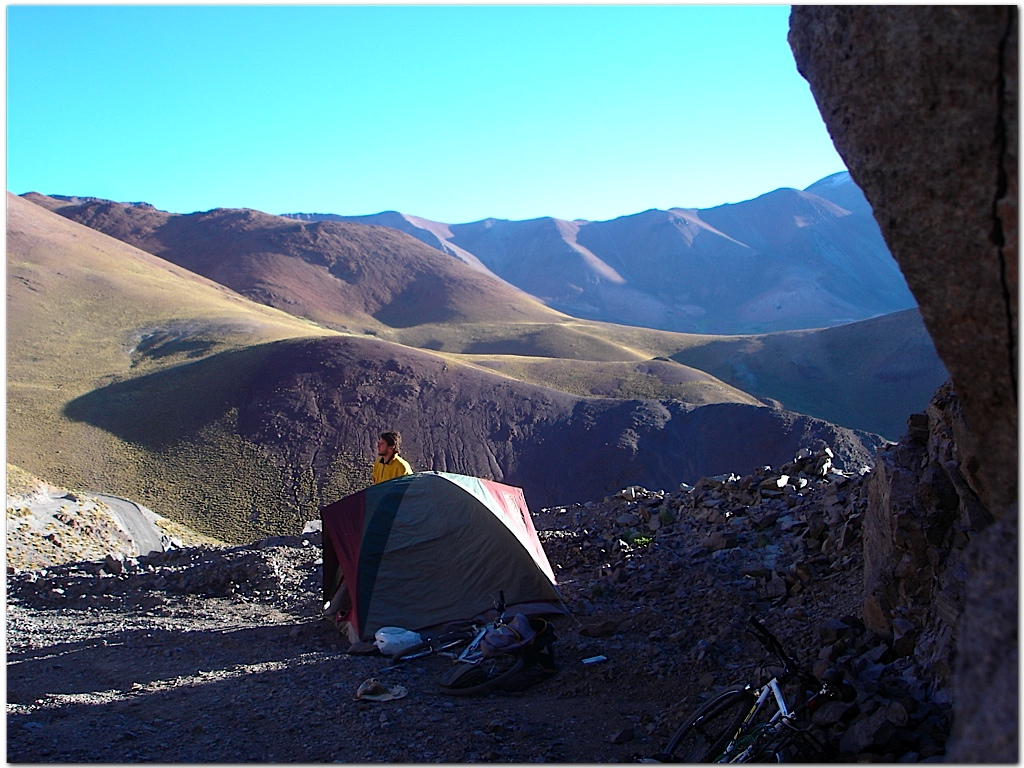
\includegraphics[width=300px]{images/DSC0375.JPG}
\textsc{\\Amanecer en el camino.} \end{center}

La otra sensaci'on que nos acompa\~naba ya fue descripta, pero intentar'e
transmitir la monoton'ia: uno sube las ``zetas'', sabiendo que luego de la curva
llega a la meta. Pero no, luego de la curva hay otra recta en subida, otra curva
m'as, y paisaje invisible desde esa perspectiva. Entonces se resigna, sigue con
la cabeza gacha, mirando hacia atr'as, o adelante seg'un el 'animo, llega la
curva, se da vuelta ansioso por ver el (\textexclamdown por fin!) Abra, pero no:
existe una nueva recta de iguales caracter'isticas. Los latidos se sienten en
todo el cuerpo. El sol abrasa. \textexclamdown Cu'anas subidas restan, Dios! Es
como si nunca se terminara, es como el juego ``viboritas'' en que la situaci'on
nunca mejora sino que empeora, a pesar de todas las frutitas que uno comi'o.
Pero lleg'o el momento en que no se ve'ia nada m'as que el cielo, y entonces era
seguro que ser'ia la 'ultima subida. Yo se que no pod'ia m'as, se que no ten'ia
energ'ias, pero se tambi'en que aceler'e imparablemente, hasta llegar a
comprobarlo. Y lo comprob'e. \textexclamdown Y hab'ia llegado! ``\textexclamdown
\textexclamdown {\small EZEQUIEL, LLEGAMOS}!!'' No m'as fr'io,
no m'as hambre, no m'as sed, no m'as cansancio. Euforia. Los Gemelos estaban
casi a nuestra altura. El camino se ve'ia desde arriba serpentear en ambos
sentidos. Era la cresta de la ola, el l'imite geogr'afico que podr'ia impedir
llegar a nuestro objetivo; era el inicio de nuestra Quebrada de Humahuaca.

Ezequiel estaba a dos curvas de distancia hacia abajo, unos 500 m. En un momento
de peligrosa confianza baj'e, no por el camino sino cort'andolo por la
monta\~na, para contarle, emocionado, que all'i mismo se encontraba el Abra, con
todos sus carteles, vistas y pompas. Hac'ia cinco minutos no serv'ia ni para
acostarme a mirar el cielo sin quedarme dormido, y ahora bajaba a ayudarlo a
empujar su bicicleta hasta el Abra; el estado emocional es tanto o m'as
importante que el f'isico, no se necesitan pruebas. Ezequiel tambi'en se
emocion'o y gan'o en energ'ias y voluntad, pero a'un se sent'ia mal
f'isicamente. Yo sub'i sin parar su bicicleta --que en estas altitudes es m'as
bien un obst'aculo-- hasta lograr posicionarla al lado de la m'ia, y lograr
``la foto'', algo incomprensible teniendo en cuenta que par'abamos a tomar aire
cada 100 metros o menos de caminata. Yo saqu'e dos fotos tontas como siempre (mi
talento fotogr'afico es cercano a nulo), y mi amigo, encargado de este aspecto,
de suerte que quiso acomodar la c'amara sobre alguna piedra para que nos
retrat'aramos juntos. Ni importaban las bicicletas. Lo 'unico que quer'iamos
luego de aquella foto de forzada pero muy alegre sonrisa, era bajar a San
Antonio, respirar, y volver a saciar nuestros vac'ios est'omagos. Debilita, la
altura, no es redundante el dato: como bichos de ciudad pampeana no lo
entend'iamos. Julio Godoy en su libro relata que en su primer gran cumbre
sinti'o\ldots\ humildad. No fue euforia, no fue orgullo, sino llana humildad
ante la enormidad que lo rodeaba.

Transitar esos 7~km nos llev'o 4 horas, muchas paradas hasta calmar pulsaciones.
\textexclamdown Los corazones hicieron m'as fuerza que las piernas!

Paisajes fenomenales, curvas, ripio, arena\ldots\ la bajada no permit'ia
aburrimiento. Si bien era muy divertido y extra\~no no pedalear para avanzar, no
era f'acil, avanzando un tanto mareados, r'apido sobre un suelo tan irregular.
Cuando llegamos a la recta (de la Nacional 40, no se lo pierdan) \textexclamdown
ten'ia tantos vados, canaletas, arena y piedras de todos los tama\~nos,
\textexclamdown que mantener el equilibrio sobre las r'apidas bicis se hac'ia
dif'icil! Cruzaban llamas a veces, se las ve'ia correr por los valles desde
arriba en el camino.

Luego de otra larga recta con fuerte viento en contra (como todos estos d'ias,
el viento) llegamos a San Antonio de los Cobres en estado de inanici'on: hac'ia
dos d'ias, casi, que no com'iamos, con todo el esfuerzo que hicimos. A las 5 de
la tarde entramos en un restaurant sin cartel a pedir comida.

\subparagraph{}\label{ssub:comerAhora} --- \textquestiondown Comida?
\textquestiondown Pero ahora? \\ --- \textexclamdown S'i! \textexclamdown
\textexclamdown Como si fuera un almuerzo o cena!!\\ \hangindent=1cm

As'i que comimos de entrada una suculenta pizza, para dejar lugar al plato
principal: una milanesa napolitana con ensalada. Dos gaseosas\ldots\
\textexclamdown comimos como si fu'eramos cuatro! ``Gracias por la merienda", le
dijimos a la buena mujer, y a instalarnos en una suerte de hostal vac'io, donde
dejaron la calefa puesta. Ba\~naditos, al cyber, postres dulces, \textexclamdown
y a dormir!

Hermosa gente encontramos por la 40. S'olo lugare\~nos, y otros dos mochileros.
\emph{Nadie} m'as. No llegamos a conocer a un ciclista ingl'es que iba un d'ia
m'as adelante que nosotros (nos llev'o un d'ia m'as de lo pensado el gran
trayecto).

\textexclamdown Bueno, eso ser'a todo, resumid'isimo aunque no lo crean! El Abra
ser'a algo dif'icil de olvidar. Lo comparaba con el cruce de la cordillera por
Mendoza, s'olo que much'isimo m'as dif'icil (ripio, arena, viento, falta de
aire, de gente y de provisiones). Y, claro, tambi'en \emph{hermos'isimo}. Las
monta\~nas que 'ibamos rodeando se iban viendo desde arriba a medida que
ascend'iamos. Se siente.

Ma\~nana, colectivo a Purmamarca: a Eze no le dan los d'ias para pedalear por
las Salinas y tambi'en llegar a Iruya, que creemos prioritario.

\textexclamdown Un abrazo enorme a todos!

Tute.

\section{Vuelven las vacaciones: hacia la Quebrada}

\subsection*{1 de Febrero}

\textexclamdown Hola, familia y amigos! \textquestiondown C'omo andan?

Llegamos a San Antonio muy cansados y hambrientos, por fin bastante aire y
suficientes alimentos. Dormimos en su oficina tur'istica a'un no oficial, y
desde aqu'i avanzar'iamos por Pozo Largo y Tres Morros, a trav'es de las Salinas
Grandes, para bajar por la Cuesta del Lip'an a Purmamarca: la Quebrada. Para
ello deb'iamos quedarnos descansando otro d'ia, y viajar a pedal otros tres,
pero las cuentas para llegar a principios de Febrero ya no daban, por lo que
aquella misma ma\~nana tomamos un colectivo a Purmamarca, con transbordo de
pocas horas en Salta (hermosa, verdaderamente). La ruta a Salta, incre'ible, y
luego nos tocaba la selv'atica ruta 9. El d'ia de descanso avanz'abamos,
\textexclamdown extra\~no!

Purmamarca es un pueblito hermoso, es famoso su cerro de los 7 colores, que se
debe llamar as'i por tener todos los colores que en la Quebrada abundan pero en
ese 'unico accidente geogr'afico. Sorprende de este poblado la uni'on de turismo
familiar y mochilero, siempre separados kilom'etricamente, pero ahora casi
compartiendo los mismos lugares. Descansamos dos d'ias: primero viajando en
colectivo, luego recorriendo los alrededores: pues no nos quisimos perder, a
pesar del cambio de ruta, las Salinas Grandes, y tomamos un colectivo para
conocerlas. La Cuesta del Lip'an fue maravillosa: el camino sube 2000 metros en
pocos~km, para bajar luego desde esos 4000 a las Salinas, a unos 3000 msnm.
Incontables curvas pavimentadas, en buen declive, y en ese marco monta\~noso.
Bajarlas en bici era sin precio, pero de verdad no podr'iamos llegar a completar
el viaje, de hacerlo. Y las Salinas\ldots\ perder la vista en esa plana s'abana
blanca y encandilante, luego de semanas de monocrom'aticas monta\~nas, fue
m'agico.

Buen sol todos los d'ias. Buen camping, buena gente. Cenando toc'o un d'uo medio
candombero espectacular, con caj'on de percusi'on, guitarra, voces y muy, muy
buena onda. Alegr'ia.

Bici a Tilcara, 20~km de viento a favor y pavimento, no podemos creer lo poco
que nos llev'o. Paramos en Maimar'a, poca gente lugare\~na, interesados en el
viaje y muy simples y abiertos. Aqu'i, la Oficina Tur'istica, la Terminal de
Omnibus y el Registro Civil, comparten un mism'isimo edificio. Mientras hablaba
con pap'a por tel'efono luego de varios d'ias sin comunicaci'on, Ezequiel
charlaba sin parar con un ni\~no que bajaba por una calle en su bici; cuando yo
cortaba ellos se desped'ian con un fuerte abrazo. Le hab'ia dejado \$2 para que
puediera ba\~narse en la pileta del club municipal, un regalo perfecto para la
calurosa tarde. \textexclamdown Creo que la sonrisa de Eze era m'as grande que
la del chico!

La Quebrada de Humahuaca es como conocer en pocas horas distintos pa'ises,
\textexclamdown todo el tiempo cambia el paisaje! Un buen viaje: el decidido
viento Sur convirti'o las subidas en planicies. Tilcara es otro lindo pueblo,
luego de recorrerlo en bici las dejamos en alg'un campamento, y subimos a pie al
Pucar'a de Tilcara, ruinas ind'igenas con vista interminable a trav'es de la
Quebrada de Humahuaca, y adelante, hacia otro valle. Los Pucar'a pod'ian ver
acercarse personas a decenas de kil'ometros de distancia, pero no aprendimos
mucho m'as sobre su historia.

Y ma\~nana, a Humahuaca: unos 40~km de buen viento Sur. Los d'ias ya aprietan,
eso no est'a tan bueno, sin embargo vamos a llegar a Iruya si todo sigue como
viene, bien.

\textexclamdown Un abrazo grande a todos!

Tute.

\subsection*{2 de Febrero}

\textexclamdown Hola a todos! \textquestiondown C'omoandan? (De nuevo noanda la
barra espaciadora.)

Che, me invitaron por mail a unirme a un apag'on de 5 minutos para solidarizarme
con el calentamiento global. \textexclamdown No saben que nos estamos
solidarizando desde hace tres semanas! Cuando lleguemos vamos a prender y apagar
la luz como ``El N'aufrago''.

Es sensacional pedalear por lugares como Humahuaca. Las angostas callecitas de
piedra, grandes plazas, casas coloniales, y los grandes faroles antiguos del
centro hist'orico de Humahuaca nos cautivaron. Adem'as, llegamos el d'ia de la
Fiesta de la Virgen de la Candelaria, mitad cat'olica mitad pagana. No
esper'abamos combinar con ninguna de las fiestas norte\~nas, fue algo
inolvidable. Hab'ia diversos grupos musicales de los alrededores, todos tocando
m'usica andina con sus tambores, sicus y otros; dos ``leones'' dando la vuelta a
la plaza tirando fuegos de artificio; cientos de turistas mirando y escuchando
extasiados; y la iglesia tocando sus campanas en plena noche y madrugada. Fue
asombroso y bien divertido. De visitar la Quebrada, hay que visitar alguna de
sus fiestas regionales.

Hab'ia mucha gente. Los sicus sonaban met'alicos, como un carrito de
supermercado que chilla, no como aire en una ca\~na; raro. Tipo 1:00
interrumpi'o una repentina y potente tormenta de verano, pero como tal se alej'o
en breves minutos. Las celebraciones comenzaron de nuevo a las 6 de la
madrugada, mientras dorm'iamos pl'acidamente. La iglesia empez'o media hora de
campanadas, todo empezaba de nuevo, sin embargo seguimos durmiendo como
lechonazos.

Nos levantamos a duras penas a las 11am, desayunamos, compramos uvas a falta de
sand'ia para el camino, y a pedalear a Chaup'i Rodeo, a mitad de camino de
Iruya, unos 45~km. Ma\~nana estaremos llegando all'a si todo va bien. Estoy
ansioso y expectante.

Vamos encontrando gente de otros campings, todos vamos al mismo paso; lo empiezo
a sentir, claro, en la Quebrada y no por la 40.

Si bien ayer en la tarde me informaron de la inminente aunque impredecible
muerte de mi abuelo, y Ezequiel me acompa\~nar'ia de vuelta en caso de querer
estar en Pergamino cuanto antes, decid'i seguir a Iruya. 'El estaba enfermo
desde hac'ia tiempo, y tuve ocasi'on de despedirme antes de mi partida. El
intercambio de palabras que mantienen un viejo ya cercano a su muerte y un
joven, donde el primero eval'ua c'omo vivi'o y c'omo vivir, desde su peque\~na
o gran experiencia. Lo enorme es la irremediable humildad desde la que habla, no
importa, justamente, su grandeza o peque\~nez en la vida que llev'o. Eso, creo,
es lo que aporta valor a esos pensamientos.

Volviendo a Humahuaca, es una ciudad cuyo centro es espectacular, bien colonial;
aunque en las afueras se parece m'as a la ciudad de Tucum'an. Ac'a todos muy
abiertos: encontramos introvertidos o caraduras por el camino; \textexclamdown
no hay lugare\~nos ``t'ermino medio''!

Contentos, a ver c'omo nos tratan las piernas en nuestro segundo tramo de
subidas en ripio. Los paisajes, dicen, prometen. La bajada a Iruya, dicen, es la
mejor frutilla del postre que hayamos podido elegir. \textexclamdown No est'a
bueno esperar tanto de una cosa, pero as'i es como estoy!

\textexclamdown Un abrazo grande a todos! \textexclamdown Cuenten como andan!
Beso grande;

Tute.

\subsection*{3 de Febrero}

\textexclamdown Hola a todos! \textquestiondown C'omo andan?

Llev'abamos un buen viaje cuando a los 20~km, la tormenta que me tocaba los
talones me desesper'o, y entr'e en Hornaditas m'as nervioso de lo que deb'ia.
Para colmo era una enorme nube pasajera que a la media hora desapareci'o (aunque
hubo otras). Lleg'o Eze y pens'o en quedarse una horita a descansar, o ``lo que
queramos'', as'i que estando de acuerdo nos echamos bajo la copa de un gran
'arbol. Hornaditas es una comunidad aborigen, este era una suerte de centro
institucional, con canchita de f'utbol, iglesia, jard'in de infantes, y un
caser'io. Nunca nos levantamos para seguir.

Estamos mal, hay algo que sentimos y no sabemos si es por altura, luego de tres
semanas de aclimataci'on: cansancio extremo, dolor de cabeza, ganas de dormir y
dormir, y de no comer porque no podemos digerir. Descans'abamos bajo un hermoso
'arbol, cuando pas'o un t'imido lugare\~no a pie, lo saludamos y si contest'o lo
hizo muy bajito. El hombre, Beto, entr'o en el sal'on de la iglesia y se nos
vino la imagen de Uspallata: ``\textexclamdown en este viaje nos falta dormir en una iglesia!''
dec'ia Eze. Al salir le pedimos alojamiento, nos ofrec'ia un sucucho bien sucio.
Luego ofici'o de gu'ia tur'istico mostrando un tremendo mirador (los colores del
cielo, irreales), el card'on m'as viejo y grande de toda la Quebrada, y nos
dec'ia que el desv'io a Iruya no tiene cartel (\textexclamdown mentira!) y que
m'as vale llegar de d'ia (era el atardecer). Sin decirlo aceptamos no
seguir viaje, as'i que fuimos a arrear unas cabras y a divertirnos con un perro
que devolv'ia los cabezazos que 'estas le tiraban. Pasamos una buena tarde, se
hizo de noche, y nos permiti'o dormir en el sal'on de la iglesia, con olor a
vino por el festival del s'abado pasado. Buen'isimo, ni carpa armamos. (A
medianoche y desesperados, s'i, \textexclamdown malditos mosquitos!)

\begin{center}
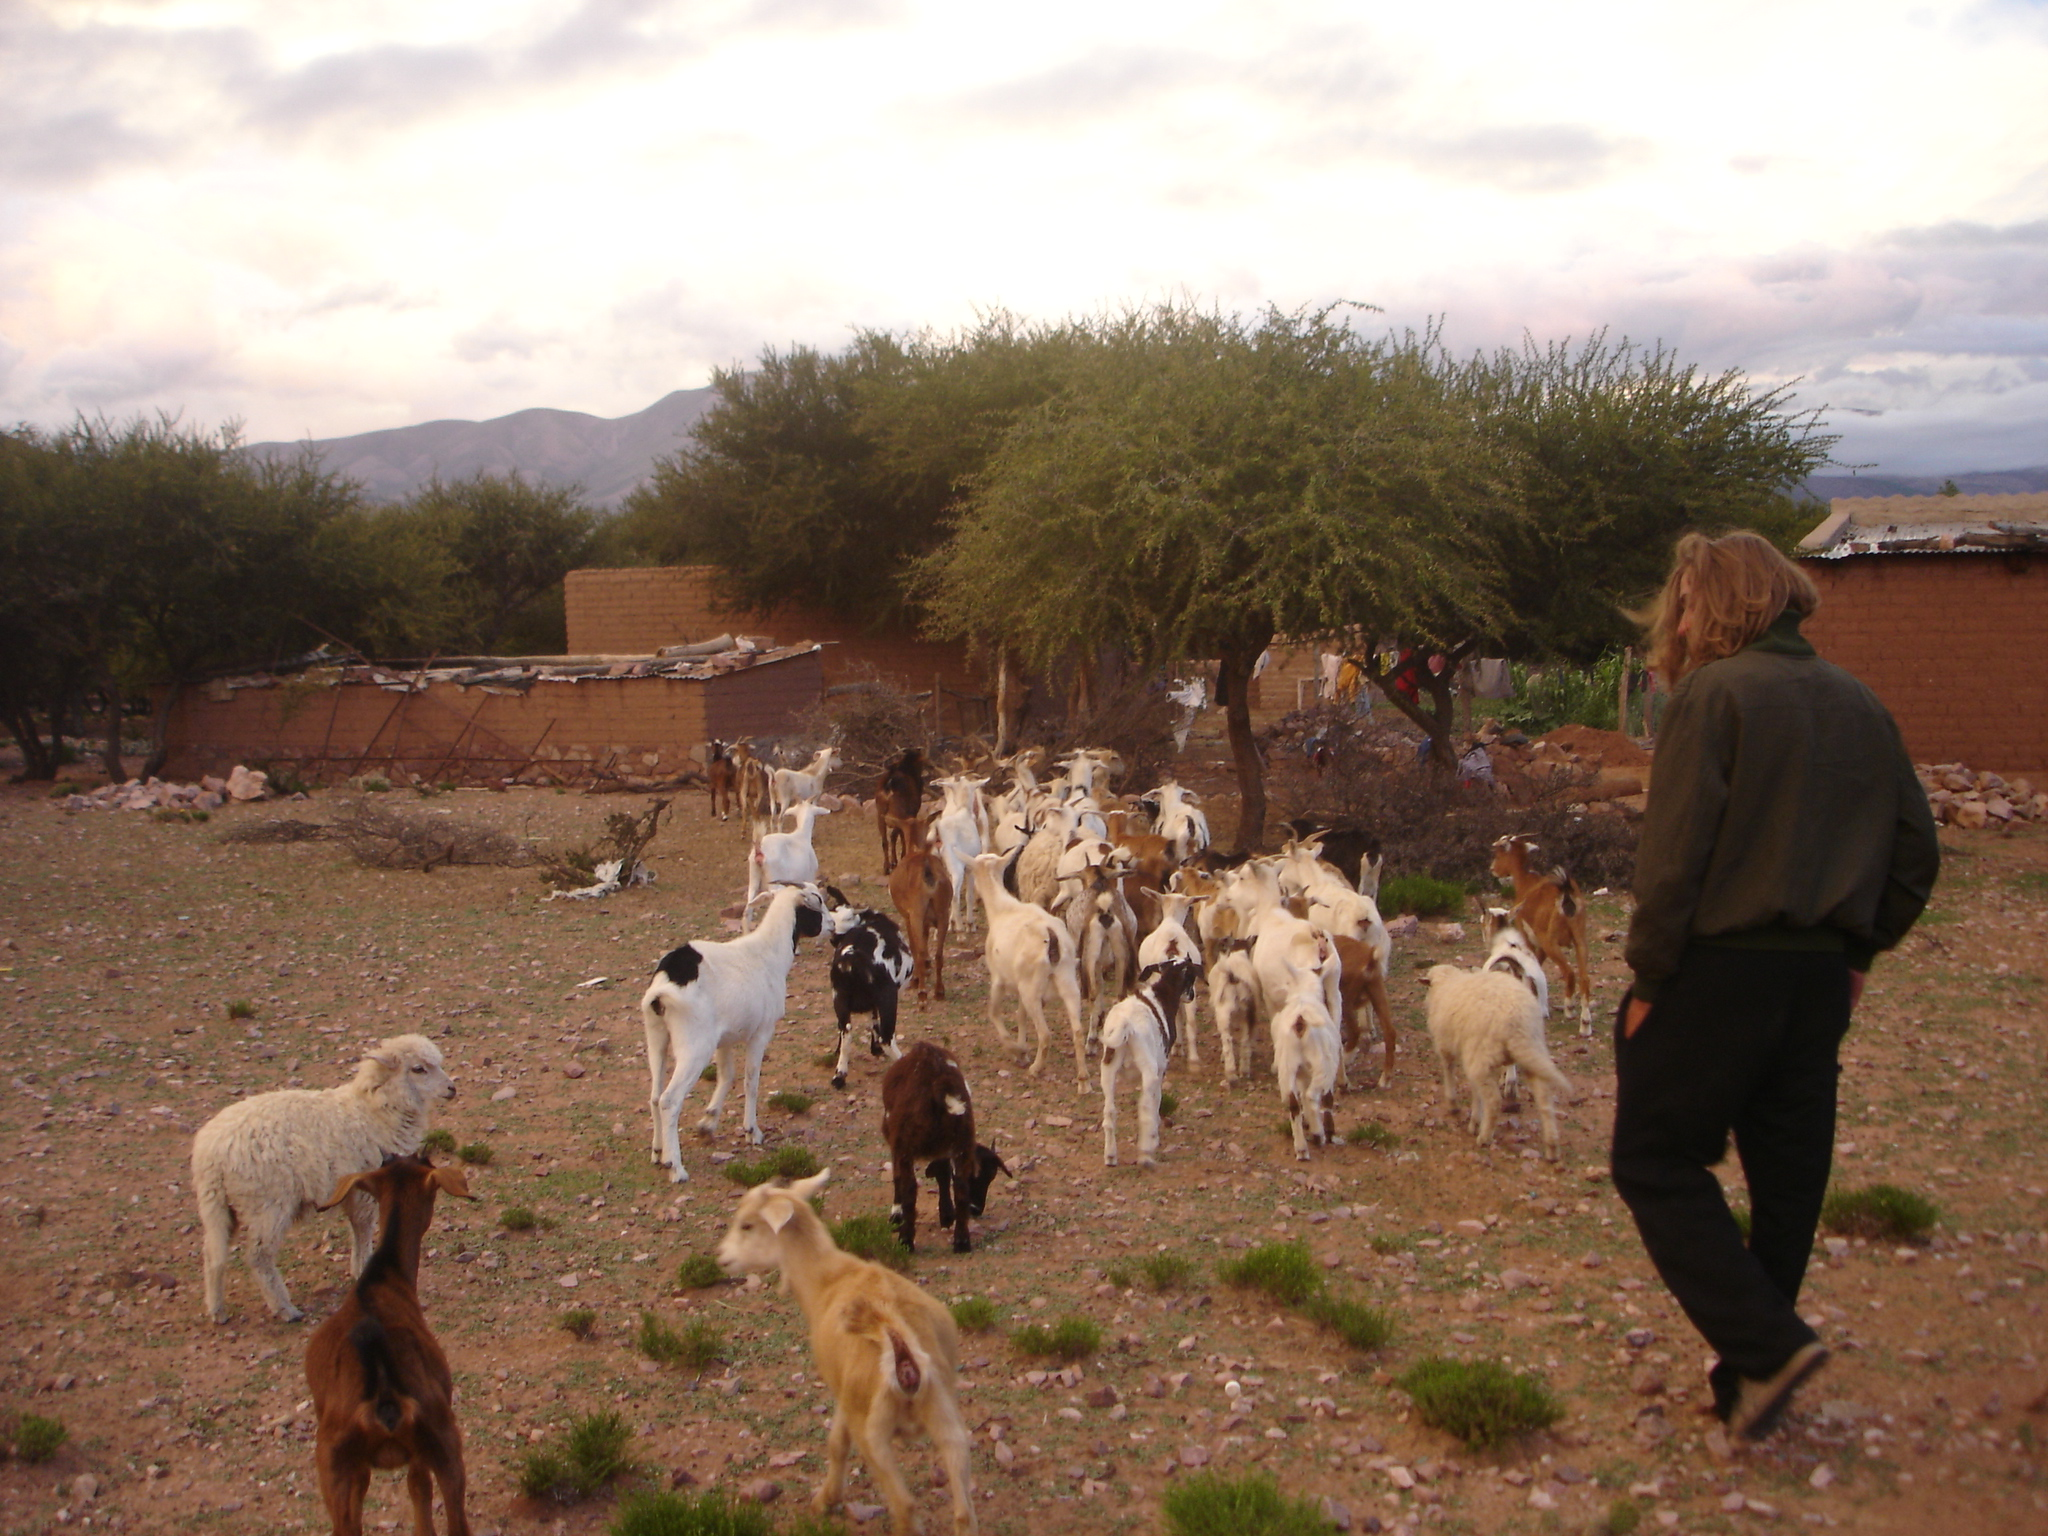
\includegraphics[width=300px]{images/DSC0446.JPG}
\textsc{\\D'ia de descanso.}
\end{center}

Cenamos poco arroz en el sal'on de la Iglesia que el muchacho nos prest'o, y ya
m'as en confianza, nos empez'o a contar de su vida. Beto es de Hornaditas, 26
a\~nos, soltero, m'as bueno que el pan lactal. Se encarga de muchas cosas, pero
oficialmente nos coment'o que de encender y apagar la bomba del agua todos los
d'ias. Pero por ejemplo, esas cabras no eran de 'el, sino del hermano, aunque lo
llamaba ``vecino''. Lo invitamos a un arroz tan rico como pudimos y, contaba que
un d'ia llegaron (es por desv'io, no es tan com'un la gente por aqu'i) dos
sacerdotes espa\~noles y le hicieron muchas preguntas que 'el contest'o con
buena predisposici'on. Tiempo despu'es les lleg'o la noticia de que la comunidad
de Hornaditas era beneficiaria de una ayuda econ'omica proveniente de no-se-qu'e
fundaci'on religiosa para que instalen la bomba de agua con su trabajo, y que
puedan dejar de llevarla en bidones de 5lts. Cumplieron tan bien que fueron
enviando m'as peticiones y se las fueron concediendo, as'i que con esa ayuda
concretaron otras cuantas obras. \textexclamdown Orgulloso el hombre de lo que
hab'ian logrado entre todos!

Un tipo muy interesante, simple, amigable y de personalidad humilde; escucha
atento las historias de todos los turistas que pasan, usualmente mochileros. No
pod'ia creer que nunca hayamos cruzado por Buenos Aires a famosos de la
televisi'on que 'el nombraba; le describimos c'omo es la Capital, comparando con
las extensiones de aquella ruta, ya que no pod'ia imaginarse la dimensi'on.
\textexclamdown Tantas personas! Tambi'en se sorprend'ia el buen hombre de que
no supi'eramos lavar ropa, ``\textexclamdown Mir'a esos cuellos!'' Claro, ese
lavarropas que nos acostumbra. Escuchaba atento el hombre, pero siempre para
conocer y de modo simple, agradable.

Luego de una charlita con 'el y una discusi'on entre nosotros decidimos tomar
los colectivos ``Mendoza'' hasta Iruya, o por lo menos al Abra del C'ondor, el
punto m'as alto del camino (4000 msnm) para hacer la bajada; ya que no nos
sentimos bien ni con ganas de hacer esa ruta de subida. Todav'ia ten'iamos que
arreglar una rueda pinchada. Nos acostamos a domir invitando a Beto al desayuno
de ma\~nana, aunque ten'iamos poca chocolatada y galletitas. Dejamos sonar el
despertador de las 7, y cuando lleg'o a las 8 se sorprendi'o de que a'un
durmi'eramos. 'El se volvi'o a Humahuaca dej'andonos desayunar, y nos sugiri'o
el colectivo de las 11. Nos levantamos, desayunamos poco, y lleg'o su hermano
mayor del festival de Humahuaca

Era un borracho que empez'o a relatar todos sus problemas, debilidades y ciertos
miedos, porque nos encontr'o amigables. Admiraba a Beto, y a mi me daban
l'astima sus muy bien aprendidos hijos. Uno, Alejandro, de unos 10 a\~nos, es el
que hace ah'i de gu'ia, y se lo notaba muy abierto, atento e interesado.
\textexclamdown Fuerte! Pero me daban l'astima por su padre, que no dej'o de
mostrarles cari\~no aunque hablaba demasiado. Mientras hablaba
seguimos organizando, descansando y nos despedimos para ir a buscar el cole.

Contentos por el rotundo cambio de planes y la gente conocida fuimos a esperar a
la banquina, un tanto nerviosos por si suben o no las bicis. Pasaron dos sin
parar haciendo se\~nas de que esper'aramos, y el tercero (van de a tres o
cuatro) par'o, as'i que las subimos. A'un nos dol'ia un poco la cabeza. Subimos
al ``Mendoza'', hermoso, de los de las publicidades de la pel'icula ``R'io
Arriba''. Le dijimos que vamos hasta el ``Abra del Condor'', no Iruya:
\textexclamdown subimos en cole y bajamos en bici! Nos permitimos la licencia.

Camino espectacular, charlando con un amigable neoyorquino jubilado, que
oportunamente se fue a otro asiento para seguir contemplando los paisajes en
silencio. Llegamos a esos 4000msnm, donde empezamos a bajar del techo las bicis.
Eso s'i que sorprendi'o al pasaje, no se esperaban que sigamos la bajada en la
bici. Todos nos deseaban suerte, una gran buena onda. ``\textexclamdown As'i
cualquiera anda en bici!'', y risas.

Ah'i, a unos 22~km de Iruya, abandonamos el colectivo para seguir en dos ruedas,
el pasaje y el conductor nos miraban sorprendidos mientras luch'abamos en el
techo para bajar las dos bicis.

Este camino es similar al de la bajada del Abra del Acay pero con buen viento,
muy divertido. A diferencia de otras bajadas que vivimos, tiene pendientes m'as
empinadas, y la bajada es ininterrumpida hasta Iruya. Tres veces llegamos a
velocidades peligrosas {\sl (adrenalina)}, y hasta en un declive saltamos con
bicis y bolsos, \textexclamdown fascinante! Llegu'e a unas ``eses'' que se
pod'ian cortar por una recta que las atravesaba por el medio. Me mand'e con una
gran sonrisa pero las m'as grandes piedras mordieron la rueda trasera, que se
desinfl'o en instantes. La cambi'e en instantes y segu'i bajando, con el
objetivo de alcanzar los colectivos. Los perdimos, el tema del equipaje llevaba
su tiempo y tuvimos que reorganizarlo porque se iba desarmando con el traqueteo.
Comparo este viaje con un rally: frenando la trasera para entrar mejor en las
``U''s, haciendo fuerza en el manubrio para que siguiera el camino que quer'ia;
rocas, piedras, canaletas, cursos de agua\ldots\ s'i, la bajada era fabulosa.
Necesito m'as fuerza en las manos.

Llegamos, vimos desde el camino aquel famoso campanario cuadrado y celeste de
Iruya, cerraba el incre'ible viaje y nos dieron ganas de cortar las cintas de la
llegada. En realidad, dos cuadras antes empezaba una intensa subida.
\textexclamdown Casi que llegamos caminando a nuestra meta final!
\textexclamdown Llegamos de suerte a'un pedaleando!

Iruya se asienta en la parte baja de la uni'on de tres valles, es decir que
est'a rodeado de altas, inmensas, paredes de piedra y tierra. Luego de caminar
todas sus calles (cansador, \textexclamdown no hay una cuadra plana!) fuimos a
descansar a una bella hoster'ia, cuatro cuadras m'as adelante (y arriba) que la
iglesia central. \textexclamdown Paramos dos veces a tomar aire camino a
nuestras camas!\\

Aqu'i pasaron cosas interesantes. Eze se intoxic'o no sabemos con qu'e, por
suerte justito al llegar a nuestra meta. El el'astico que sostiene todo mi
equipaje se cort'o dos veces\ldots\ \textexclamdown llegados a Iruya! Es decir
que ya pod'iamos volver tranquilos.

Recorrimos poco Iruya, no conocimos mucho. Nos perdimos una caminata por el r'io
hasta San Isidro que plane'abamos hacer. Caminar las calles del poblado no
llev'o demasiado tiempo, y la verdad es que ya ten'ia ganas de volver. Hoy
Domingo tomamos un cole de vuelta a Humahuaca. Y desde aqu'i combinar'iamos con
Salta y Pergamino, pero hay un colectivo que sale derecho de Humahuaca a
Rosario, y como ya estaba ansioso, lo tomamos. Lo 'unico que me queda en el
tintero, y no es poca cosa, es conocer mejor Salta capital. Pero es lo 'unico
porque de la ruta, \textexclamdown todo concretado! Contentos.

En el viaje a nuestras Pampas comenzamos a ver verde de nuevo; planicies, y
'arboles\ldots\ se extra\~naban. \textexclamdown Ya no vemos piedras y rocas en
las banquinas!

Contentos de haber recorrido todo el viaje. Nos llev'o casi un mes, poco m'as de
600~km. Super'o las altas expectativas. Grandes vivencias.

\section{Hogar, dulce hogar}

\textexclamdown Me doy la bienvenida a la civilizaci'on! Qu'e hermoso es volver.
Placenteramente ocup'e buena parte de mis primeros d'ias en ba\~narme, comer,
tomar las aguas y gaseosas que quise, visitar queridos, conducir veh'iculos,
arreglar la bici, cambiar de ropas a diario, meterme en la pileta (pero no tomar
sol), salir de noche, dormir en s'abanas\ldots\

Extra\~n'e profundamente cada simpleza que ennumero, y sin embargo en la vida
all'a con la bici y mi amigo disfrut'e tant'isimo como ahora, adoptando aquello
por normal y todo esto como lujo. Esa es la sensaci'on que me invaden los
Febreros de cada a\~no, y \emph{me encanta}.

Una de mis razones para tomar estos viajes exigentes. Volver, y amar todo lo
cotidiano como la primera vez, como un buen ni\~no. Ahora me toca aterrizar, y
decantar todo lo vivido.

\newpage
\thispagestyle{empty}